%
%  generation_talk
%
%  Created by Mark Eli Kalderon on 2011-10-04.
%  Copyright (c) 2011 Mark Eli Kalderon. All rights reserved.
%
%  Beamer

% Definitions and macros
\newcommand{\change}{\textcolor{blue}{\textbf{CHANGE SLIDE}}}
\newcommand\myauthor{Mark Eli Kalderon} 
\newcommand\mytitle{The Generation of the Hues}
\newcommand\myinstitution{University College London}

% Packages specific to lecture notes
\mode<article>{
    \usepackage{palatino}
	\usepackage{setspace}
	\doublespacing
}
\mode<beamer>{
\setbeamertemplate{navigation symbols}{}
}

% Packages common to lecture notes and beamer presentation
\usepackage{pgf}
\usepackage{tikz}
\usepackage{hyperref}


\setjobnamebeamerversion{generation_talk.beamer}

\title{\mytitle}

\author{\myauthor}
\institute{\myinstitution}

\date{}

\begin{document}

\frame{\maketitle}

The presence of the fiery substance illuminates the transparent me\-di\-um. White (\emph{leukon}) corresponds to the presence of this determinant of what is actually transparent. Conversely, black (\emph{melaton}) corresponds to its absence. The absence of the fiery substance darkens the transparent medium. White and black are thus associated with a fundamental condition on the visibility of remote external particulars. No doubt in part because of this Aristotle attempts to explain the other hues in terms of the ratio of white and black. He considers three such accounts, in terms of (1) juxtaposition, (2) overlap, and (3) mixture, advocating the third. On all three accounts chromatic hues are determined by white and black in various ratios, the accounts differing only in how these ratios are implemented. 

The fundamental idea common to all three accounts can seem surprising. How can the ratio of white and black result in something appearing red? Would it not instead appear gray? Thus Hett complains that Aristotle's ``doctrine could hardly have survived a few experiments with pigments''. But if Aristotle's account were disconfirmable by elementary experimentation, then why did he not investigate the matter? Was it merely to avoid Plato's charge of impiety? (Number 1 on your handout.) Aristotle's account of the generation of the hues may be surprising, but it would be wrong to prematurely dismiss it. 

The first thing to observe is that \emph{leukon} and \emph{melaton} are better understood as light and dark, rather than white and black. There is a general tendency in Greek color vocabulary to classify colors in terms of relative brightness rather than hue. Traces of such a usage exist in English. Thus we speak of white wine and white people, though neither are white in hue. This usage in English, however, doesn't seem to be perfectly general but is rather lexically determined. ``White'' can be interpreted in terms of relative brightness instead of hue only when applied to certain nouns. The more general usage in Greek is philosophically significant, for it transforms Aristotle's claim. Aristotle is not claiming that the hues are determined by the ratio of white and black, but that they are determined by the ratio of light and dark. Experiments with pigment mixtures are irrelevant to the truth of this latter claim. Thus, Aristotle need not have risked Plato's charge of impiety as Hett recommends. 

Two further considerations are relevant. First, there are a range of observable phenomena that support Aristotle's fundamental claim that a ratio of white and black can give rise to chromatic appearances. Second, Aristotle's account has ancient precedent. Thus when Theophrastus discusses Democritus's view that there are four primary colors, he contrasts it with the then dominant view that white and black are the two primary colors. It is reasonable to suppose that Aristotle's account draws on this pre-Democritean tradition. Thus before discussing Aristotle's account, I will review some empirical support for its central idea, and will discuss the precedent for this doctrine in Parmenides and Empedocles. \change

\begin{frame}[t]\frametitle{Benham's Disk}
	\begin{center}
		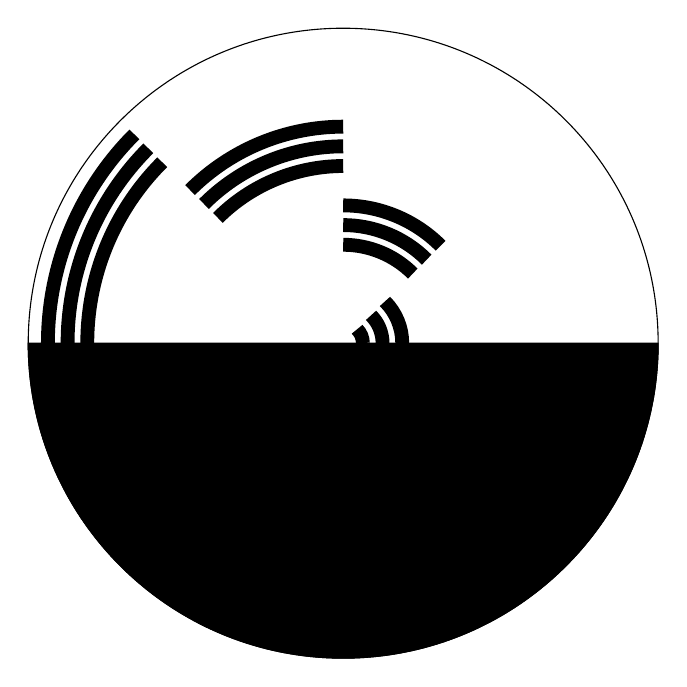
\begin{tikzpicture}
			\draw (0,0) circle (4cm);
			\filldraw[fill=black] (0,0) -- (4cm,0cm) arc (0:-180:4cm) --cycle;
			\draw[line width=5pt] (canvas polar cs:angle=0,radius=0.25cm) arc (0:45:0.25cm);
			\draw[line width=5pt] (canvas polar cs:angle=0,radius=0.50cm) arc (0:45:0.50cm);
			\draw[line width=5pt] (canvas polar cs:angle=0,radius=0.75cm) arc (0:45:0.75cm);
			\draw[line width=5pt] (canvas polar cs:angle=45,radius=1.25cm) arc (45:90:1.25cm);
			\draw[line width=5pt] (canvas polar cs:angle=45,radius=1.50cm) arc (45:90:1.50cm);
			\draw[line width=5pt] (canvas polar cs:angle=45,radius=1.75cm) arc (45:90:1.75cm);
        	\draw[line width=5pt] (canvas polar cs:angle=90,radius=2.25cm) arc (90:135:2.25cm);
			\draw[line width=5pt] (canvas polar cs:angle=90,radius=2.50cm) arc (90:135:2.50cm);
			\draw[line width=5pt] (canvas polar cs:angle=90,radius=2.75cm) arc (90:135:2.75cm);
			\draw[line width=5pt] (canvas polar cs:angle=135,radius=3.25cm) arc (135:180:3.25cm);
			\draw[line width=5pt] (canvas polar cs:angle=135,radius=3.50cm) arc (135:180:3.50cm);
			\draw[line width=5pt] (canvas polar cs:angle=135,radius=3.75cm) arc (135:180:3.75cm);
		\end{tikzpicture}
	\end{center}
\end{frame}

In 1894, an English toy maker, Charles Benham, devised a top adorned with a black and white pattern. Sold through Messrs. Newton and Co., an announcement of the ``Artificial Spectrum Top'' was published in \emph{Nature} where the ``curious point'' was raised:
	\begin{quote}
		\ldots\ that when this disc is revolved, the impression of concentric circles of different colors is produced upon the retina. If the direction of rotation is reversed, the order of these tints is also reversed. 
	\end{quote}
Each of the spinning arcs reflect light with the same spectral content and with equal average luminance. Before observing the spinning disk, one might reasonably expect the spinning arcs to appear as gray rings of equal brightness. Why, then, do the rings appear reddish, greenish, light blue, and violet? The subjective colors of the Benham disk are not completely understood. However, this much is clear: The innermost ring appearing reddish is the result of the visual system integrating temporal inhomogeneities presented by the spinning disk. Presentations of black and white stimuli altering at a particular temporal ratio elicits a chromatic response in normal human perceivers. \change

\begin{frame}[t]\frametitle{The Butterfield Encoder}
	\begin{center}
		
\includegraphics[height=8cm]{../../graphics/color_encoder.jpg}
	\end{center}
\end{frame}

This basic principle was used in an early prototype of color television. Developed by James Butterfield, the Butterfield encoder produces a monochromatic signal that when broadcast and displayed on a black-and-white monitor presents a chromatic appearance. The Butterfield encoder extracts a monochromatic signal from the colored scene by passing the light from the scene through cyan, magenta, and yellow filters. The filters themselves are arranged in, what is in effect, a modified Benham Disk. The bottom half of the filter is opaque with the colored filters fanned across the top half. The filters thus form a disk which is rotated. A colored object will appear black when seen through a filter of a complementary color. This and the opaque half of the rotating disk produces a pulsed black-and-white signal that elicits a chromatic response in normal human perceivers. The system produced good skin tones but unmixed hues, especially red, tended to flicker.

The chromatic appearance is once again the result of the visual system integrating temporal inhomogeneities. However, these temporal inhomogeneities are not the result of spatial movement of the object of perception, but rather due to the qualitative alterations over time of a stationary object. Each involves the presentation of white and black stimuli altering at a particular temporal ratio eliciting a chromatic response in normal human perceivers. They differ in how that temporal ratio is implemented---by the motion of an object whose parts qualitatively differ or by the qualitative alteration over time of a stationary object. \change

\begin{frame}[t]\frametitle{Bridget Riley}
	\begin{center}
		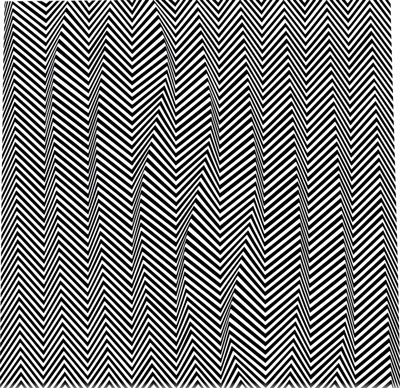
\includegraphics[height=8cm]{../../graphics/descending.jpg}
	\end{center}
\end{frame}

Stated so abstractly it is easy to see that there is a third possibility. If the temporal ratio that determines a chromatic appearance can be implemented by the motion of a black and white object, the perceiver's motion relative to a black and white object should do so as well. And indeed it can. Our eyes constantly scan the scene with involuntary saccades. Scanning a stationary black and white object can give rise to chromatic appearance. Thus Sorabji observes that contemporary art provides an example:
\begin{quote}
    The English painter, Bridget Riley, has produced pictures in which black and white are juxtaposed, in long ribbons \ldots\ When people look at these black and white ribbons, many are able to see all sorts of colours appearing.
\end{quote}
These chromatic appearances are the result of the visual system integrating temporal inhomogeneities that result from the eye involuntarily moving across a stationary black and white object. \change

\begin{frame}
	\begin{center}
		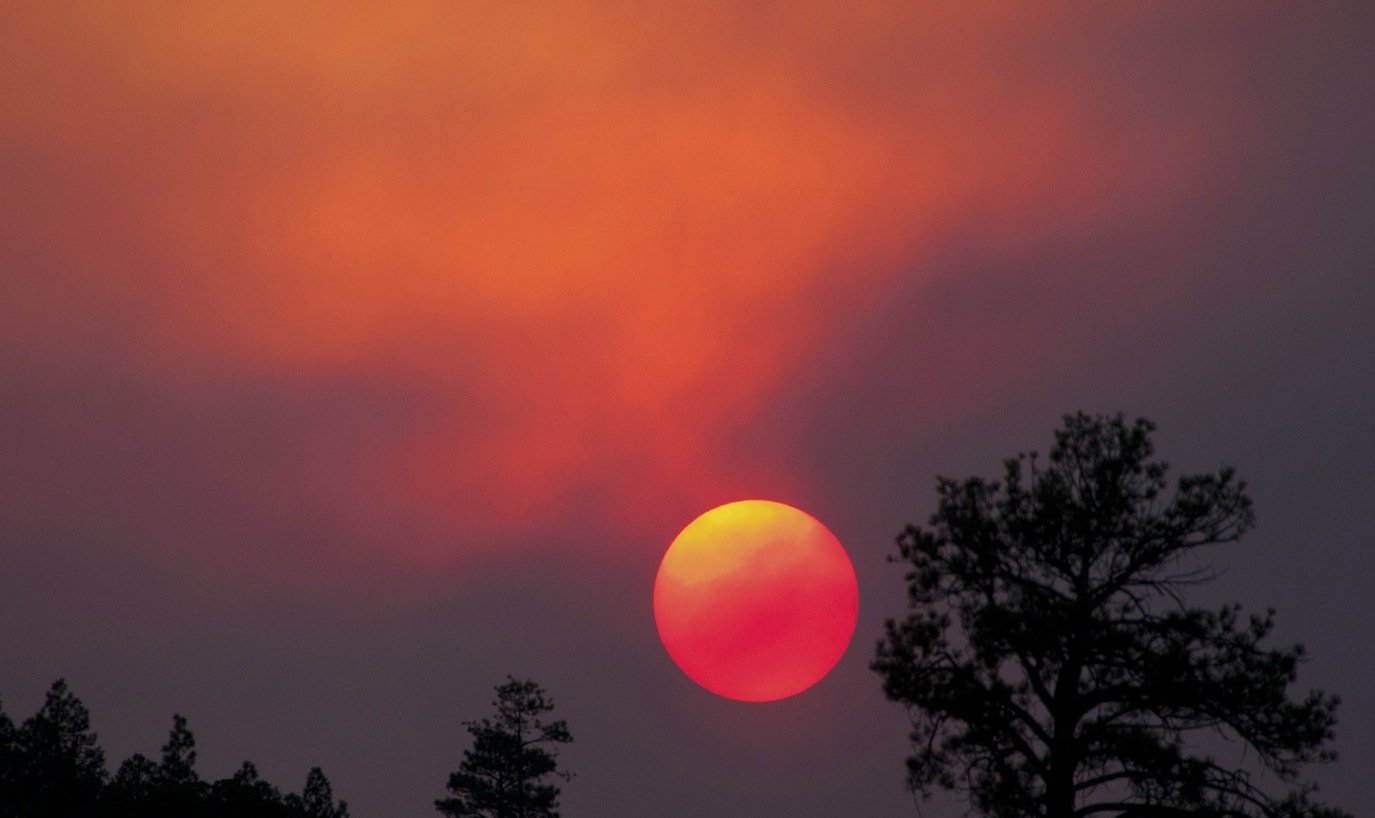
\includegraphics[height=6cm]{../../graphics/red_sun.jpg}
	\end{center}
\end{frame}

These examples involve artifacts and technology unavailable at Aristotle's time. And while they may make plausible for \emph{us} that ratios of white and black can, sometimes at least, give rise to chromatic appearances, they could not have done so for Aristotle. What empirical observation available to Aristotle could have made vivid for him the possibility that chromatic appearances are the result of the ratio of light and dark in the perceived scene? The white sun, when superimposed by black smoke, looks red (\emph{De Sensu} 3 440\( ^{a} \)10--11). And it is the reduction of the sun's brilliance by the intervening particulate matter that results in the sun's crimson appearance. This provides direct support for the claim that a proportion of light and dark can give rise to a chromatic appearance. \change

\begin{frame}[t]\frametitle{Parmenides}
	
\end{frame}

Theophrastus (\emph{De Sensibus} 79; DK 68\textsc{a}135) alludes to a pre-Democritean tradition according to which white and black are the primary colors. While Theo\-phra\-stus does not name any particular thinker belonging to this tradition, one may reasonably speculate. In his notorious study, among the five ``signs of the immaturity'' of the Homeric color scheme, Gladstone cites the following:  
\begin{quote}
    The vast predominance of the most crude and elemental forms of colour, black and white, over every other, and the decided tendency to treat other colours as simply intermediate modes between these two extremes. 
\end{quote}
Arguably, then, the pre-De\-mo\-cri\-tean tradition that Theophrastus alludes to has Homeric roots. Let's selectively examine this ancient tradition by attending to two key figures familiar to Aristotle, Parmenides and Empedocles.

In the prologue to his poem, the goddess promises to reveal to Parmenides two things, the Way of Truth and the Way of Mortal Opinion. The doctrines of the latter she assures him are false; nevertheless, Parmenides must learn these too (DK 28\textsc{b}1 31). The Way of Mortal Opinion is an account of the world ``as it appears'' (DK 28\textsc{b}8 60), and the goddess presents it to Parmenides ``so that no mortal opinion may ever overtake'' him (DK 28\textsc{b}8 61). The Way of Mortal Opinion is a cosmology in the Milesian tradition, though Parmenides is not expounding the views of any particular Milesian cosmologist. Rather, he is presenting what is, by his lights, the best account that can be given along those lines. Traditional Milesian cosmologies tend to be monistic, but the Way of Mortal Opinion posits two fundamental and irreducible principles that stand in opposition, Fire and Night (DK 28\textsc{b}8 53--61, 28\textsc{b}9). Having shown, in the Way of Truth, that monism is inconsistent with appearances, the Way of Mortal Opinion must posit a plurality of principles in opposition, if it is to accommodate the plurality and opposition encountered in the sensible world.

The two principles have attributes called ``signs''. Like Fire and Night themselves, their attributes stand in opposition. Fire is bright, Night is dark; Fire is rare, Night is dense, and so on. These attributes are sensible qualities arrayed in opposing pairs of contraries. In contrast, the attributes of the one being of the Way of Truth are not sensible but intelligible properties. Fire and Night may have further attributes not listed here; much of the Way of Mortal Opinion is missing. A sense of its scope and ambition, however, is provided by Plutarch (number 2 on your handout):
\begin{quote}
    But Parmenides \ldots\ has actually made a cosmic order, and by blending as elements the light and the dark produces out of them and by their operation the whole world of sense. Thus he has much to say about earth, heaven, sun, moon, and stars, and has recounted the genesis of man. (Plutarch, \emph{Adversus Colotem} 1114 b--c)
\end{quote}
If, according to the Way of Mortal Opinion, the whole world of sense---in which appear ``earth, heaven, sun, moon, and stars''---is ultimately explained in terms of light and dark in opposition, then the colors are themselves to be explained in terms of the ``blending'' of light and dark. Whether or not Theophrastus had Parmenides in mind, Parmenides straightforwardly belongs to the pre-Democritean tradition that postulates light and dark as the primary colors. \change


\begin{frame}[t]\frametitle{Empedocles}
	
\end{frame}

% It is at least arguable that Theophrastus did in fact have Empedocles in mind when alluding to this pre-Democritean tradition. Despite extensive discussion of Empedocles' views about sensory experience and its objects, Theophrastus does not make the parallel charge against Empedocles that he makes against Democritus (\emph{De Sensibus} 79; DK 68\textsc{a}135). This is defeasible evidence that Theophrastus took Empedocles to be among the thinkers who take white and black as the primary colors.

In contrast with Parmenidean monism, Empedocles postulates the existence of four ``roots'' or elements---water, earth, air, and fire---and two principles---\-Love and Strife. Whereas Love, the principle of harmony, has the power to unite, Strife, the principle of disorder, has the power to divide. According to Empedocles, things are colored because of the combination of elements that result from Love overcoming Strife to the extent that it does (number 3 on your handout):
\begin{verse}
    And if, concerning these things, your conviction is in any way wanting,\\
    as to how from the blending of water and earth and aither and sun\\
    the forms and colours of mortals came to be,\\
    which have now come to be, fitted together by Aphrodite.
    (DK \textsc{b}71)
\end{verse}

Wright suggests that the reference to form and color is a deliberate echo of an earlier fragment (number 4 on your handout):
\begin{verse}
    As when painters adorn votive offerings,\\
    men well-learned in their craft because of cunning,\\
    and so when they take in their hands many-coloured pigments,\\
    mixing them in harmony, some more, others less,\\
    from them they prepare forms resembling all things,
    making trees and men and women\\
    and beasts and birds and water-nourished fish\\
    and long-lived gods, first in their prerogatives.\\
    In this way let not deception overcome your thought organ\\
    that the source of mortal things, as many as have become obvious---countless---is anything else,\\
    but know these things clearly, having heard the story from a god.\\ 
    (DK \textsc{b}23)
\end{verse}
However, the two fragments seem to be making different points. Empedocles in this earlier fragment describes the generation of the objects we encounter in the sensible world by analogy with painting. Just as painters can represent everything in the sensible world by combining pigments in various proportions, Love and Strife can generate everything in the sensible world by combining the elements in various proportions. However, unlike the later fragment (DK \textsc{b}71) no specific mention is made about the colors of the generated objects or how they are the result of the combination of elements.

The painting analogy remains instructive. It sheds light on the sense in which the combination of a few colors suffice to represent the colors that appear in the sensible world. This is important since in the context of Empedocles' analogy, this is the sense in which the elements combine. And given the latter fragment (DK \textsc{b}71), the elements when combined in this sense suffice for the form and color of all things. First, observe that, despite their manifest plurality, elements are otherwise Parmenidean beings---they do not admit of alteration, growth, or decay. Change as we experience it is the result of different combinations of these unchanging elements. So for the analogy to hold, the painter's combination cannot be understood as a mixture. If when the elements combine they do so in a mixture, then the elements would no longer be distinguishable in the compound. But this is inconsistent with their status as Parmenidean beings. So a negative lesson, then, is that the combination as it figures in the analogy cannot coherently be understood as mixture.

If combination, here, cannot coherently be understood as mixture, how, then, is it to be understood? Recent commentators have made the important suggestion that combination as it figures in the analogy should be understood in terms of the actual practices of fifth century \textsc{bc} painting. However, this yields two distinct models, and as a consequence, I am less certain about the positive lessons that the analogy affords us. \change

\begin{frame}
	\begin{center}
		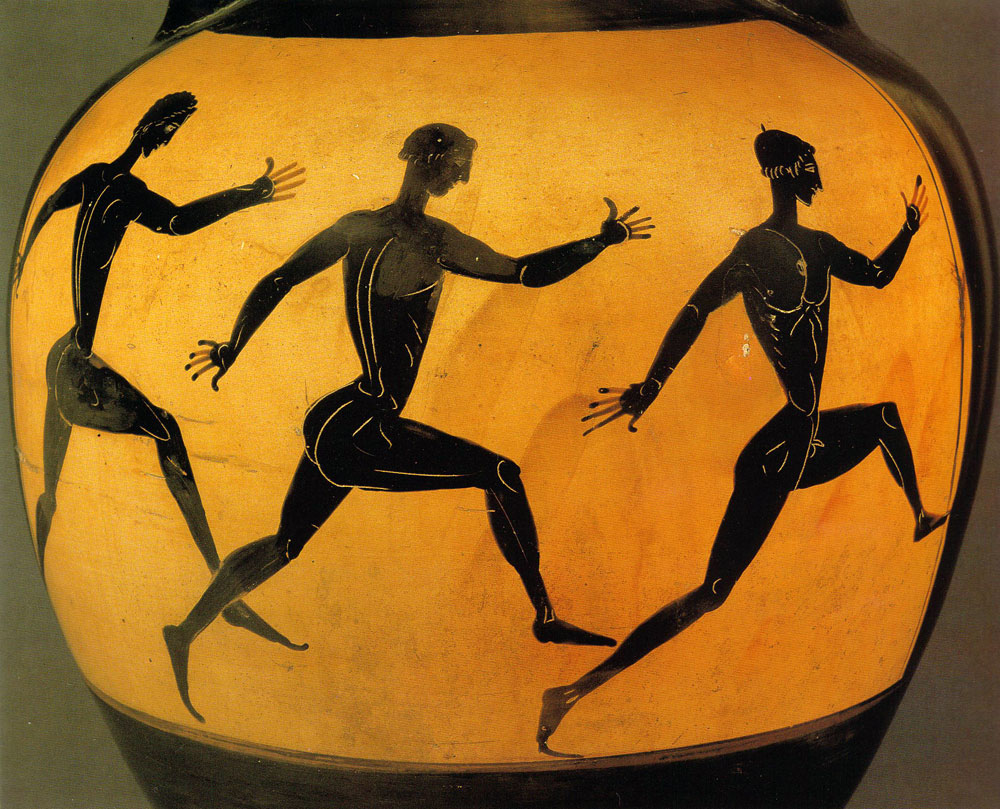
\includegraphics[height=8cm]{../../graphics/archaic.jpg}
	\end{center}
\end{frame}

Consider what is arguably the most important development of fifth century \textsc{bc} painting, the development of chiaroscuro or \emph{skiagraphia}. In archaic Greek painting, figures appear outlined and uniformly colored in a two-dimensional pictorial plane. Moreover, the color of the figures tended to complement and support the overall two-dimensional composition. \change

\begin{frame}
	\begin{center}
		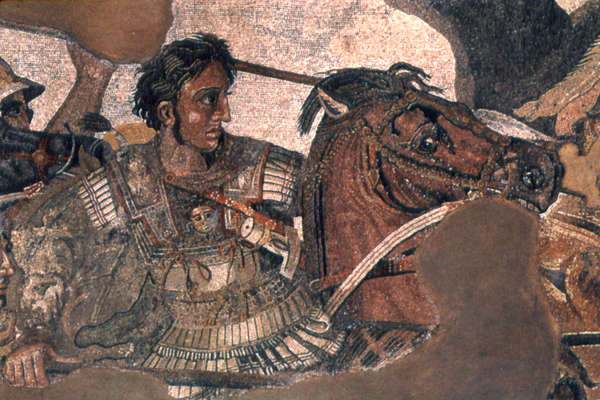
\includegraphics[height=7cm]{../../graphics/alexander.jpg}
	\end{center}
\end{frame}

However, in the fifth century \textsc{bc}, the ``shadow painters'' came to emphasize, instead, lightness and darkness in organizing their compositions. There was less reliance on outlining, figures were no longer uniformly colored as primitive methods of shading were developed, and as a result, the figures began to emerge from the two-dimensional pictorial plane. To emphasize the importance of relative brightness in their composition, the shadow painters worked with a limited palette. Nevertheless, they were able to produce the appearance of a variety of colors by combining the colors of this limited palette. Importantly, there were two techniques for combining the few colors, corresponding to different periods in the development of \emph{skiagraphia}.

Plutarch attributes the invention of fifth century \textsc{bc} chiaroscuro to Apollodorus. In seeming contradiction to this, Quintillian claims that a student of Apollodorus, Zeuxis, invented the law of light and shadow. Bruno reconciles these apparently conflicting claims by arguing that they are in fact describing distinct dramatic episodes in the development of fifth century \textsc{bc} chiaroscuro.

Not only does Plutarch attribute the invention of \emph{skiagraphia} to Apollodorus, but also the invention of a method of color combination. Specifically, working with a limited palette, Apollodorus would produce novel colors by overlaying washes of different colors, and a four-color palette was common in the fifth century \textsc{bc}. So one way of combining colors is by overlaying differently colored washes, that is, by overlap.

The more painterly style of Zeuxis involved a different method of color combination. In the late development of fifth century \textsc{bc} chiaroscuro, as light and dark came to further dominate the compositional scheme, the relationship between form and color became complicated. Whereas earlier forms of chiaroscuro would use one color for shaded parts of a figure, later forms would use a variety of colors, their choice controlled more by relative brightness than hue. The effect of this more complicated scheme may without too much risk of anachronism be described as proto-impressionistic. However, there need be no ancient predecessor of Suerat in fifth century \textsc{bc} painting for there to be a method of color combination that involved not the overlap but the juxtaposition of color.

We have seen that combination in Empedocles' painting analogy cannot be understood in terms of mixture. Fifth century \textsc{bc} painting, however, provides us with two further models. Perhaps the combination could be understood, not in terms of mixture, but in terms of overlap or juxtaposition. 

Aristotle claims that the Empedoclean elements combine by means of juxtaposition and compares the compound to a brick structure. If we accept the Aristotelian interpretation, then the combination of the elements should be understood on the model of juxtaposition. So, for the analogy to hold, the painter's method of combining colors must itself be understood on the model of juxtaposition, a method arguably associated with the late chiaroscuro inaugurated by Zeuxis. However, Zeuxis' achievement is too late---it arguably post-dates the composition of Empedocles' poem. Wright, following Guthrie, associates the painter's combining of colors with Apollodorus and Greek four-color painting, but that technique works by overlap, not juxtaposition. It is this mismatch that makes me uncertain what positive lessons Empedocles' analogy can provide us. It is possible that Aristotle is right that the Empedoclean combination of elements should be understood on the model of juxtaposition \emph{and} that Wright has correctly interpreted the painter's combination of colors in terms of overlaying washes. In which case, the analogy, considered by itself, could serve only to establish the original negative lesson. The combination of the elements is like the combination of the colors in that neither should be understood in terms of mixture. Rather, as it turns out, they work on the models of juxtaposition and overlap, respectively.

Some commentators attribute to Empedocles the view that the four elements have four unique colors. However, the fragments provide no direct support for this interpretation. While Empedocles claims that fire is white and water is black, no specific colors are associated with the other elements. I believe that it is more likely that Empedocles is following Parmenides in taking light and dark as the primary colors. To illustrate this alternative, let's consider two fragments where Empedocles' associates white with fire and black with water. \change

\begin{frame}
	\begin{center}
		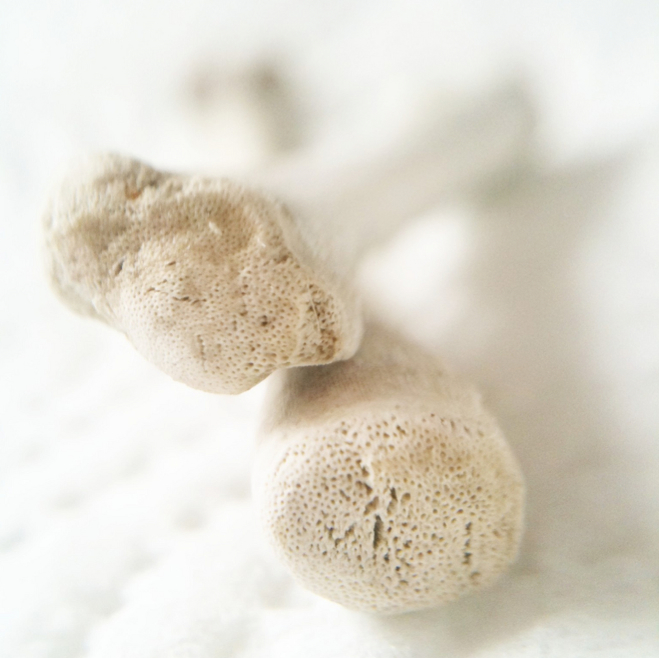
\includegraphics[height=8cm]{../../graphics/bone.jpg}
	\end{center}
\end{frame}

Aristotle cites the following Empedoclean fragment to illustrate the way in which compound bodies do not merely consist in their constituent elements, but must be combined in a certain proportion (number 5 on your handout):
\begin{verse}
    And pleasant earth in her well-built channels\\
    received two parts of gleaming Nestis out of the eight\\
    and four of Hephaistos; and they become white bones\\
    fitted together with the divine glues of harmony.\\
    (DK \textsc{b}96)
\end{verse}
Nestis is a Sicilian water-goddess, and Hephaistos is associated with fire. Thus, according to the fragment, bone is the result of Love's combining four parts fire with two parts earth and two parts water. Empedocles here seems to be explaining the whiteness of bone in terms of the preponderance of fire in its constituent elements. If we combine this thought with the answer in the style of Gorgias presented in the \emph{Meno}, then the idea would be that bone, due to the preponderance of fire in its composition, gives off a fiery effluence. This fiery effluence, due to its distinctive magnitude, enters the fire passages in the membrane of the eye and so is made palpable to sight. \change

\begin{frame}
	\begin{center}
		
\includegraphics[height=8cm]{../../graphics/black_river.jpg}
	\end{center}
\end{frame}

That fire and water are the elemental equivalents of light and dark is further confirmed by a fragment cited by Plutarch (number 6 on your handout):
\begin{verse}
    And in the depths of the river a black colour is produced by the shadow,\\
    and in the same way it is observed in cavernous grottoes.\\
    (DK \textsc{b}94)
\end{verse}
The fragment only explicitly claims that the depths of the river is black, but Plutarch cites the fragment in answer to the question ``Why does the surface of the water look white and the depths look black?'' (number 7 on your handout):
\begin{quote}
    Is it because the depth is the mother of blackness inasmuch as it blunts and weakens the sun's rays before they can get to it? But since the surface is immediately affected by the sun, it is reasonable that it receives the gleam of light.  (\emph{Historia Naturalis} 39)
\end{quote}
This supports the elemental equivalence of fire and water with light and dark. It also strikingly prefigures the central thought of Aristotle's account of the generation of the hues. Water is by nature black. However, the color that water appears to have can change depending on whether and to what degree it is illuminated. The surface of water looks white, at least in the shifting pattern of reflective highlights. The water near to the surface, where it is not as brightly illuminated, looks blue. And the depths of the river, where the sun's rays fail to penetrate, looks black. The different colors---white, blue, and black---are due to different different proportions of fire and water. In the shifting pattern of reflective highlights, there is a preponderance of fire and this results in a brilliant appearance; whereas, in the depth of the river, there is a preponderance of water (and perhaps no fire at all) and this results in a dark appearance. In the shallows of the river, due to a more equitable combination of fire and water, a blue appearance is manifest.

Accepting Plutarch's attribution, and generalizing it, thus results in the following picture: White and black, like hot and cold, are sensible qualities paired with their contrary. And like hot and cold, white and black are the endpoints of an ordered range of sensible qualities. Blue is a sensible quality located somewhere between the extremes of white and black as is every other color. Blue is perhaps more dark than light just as yellow is more light than dark. Moreover, the relevant proportion of light and dark is determined by the substance's elemental composition. The proportion of light and dark that results in the blue of the river's shallows is determined by the proportion of fire and water in its composition.

This constitutes a means for addressing Theophrastus' complaint. Theo\-phrastus concedes that on Empedocles' account, the perception of white and black is relatively straightforward. In the membrane of the eye there are alternating passages of fire and water. White effluences emitted from distal objects are assimilated by fire passages, black effluences are assimilated by water passages, and so each is made palpable to the organ of sight. But how, on this model, is the perception of the chromatic hues to be explained? (Number 8 on your handout):
\begin{quote}
	For he assigns their perception neither to the minute passages of fire nor to those of water nor to others composed of both these elements together. Yet we see the compound colours no whit less than we do the simple. (\emph{De Sensibus} 17)
\end{quote}

It is true that the perception of blue is not assigned to the fire passages, nor to water passages. Whether it is explained in terms of ``others composed of both these elements'' depends on what exactly Theophrastus means here. Perhaps he means that just as there are fire and water passages in the membrane of the eye, there are other passages, as well, that are commensurate with effluences compounded out of fire and water. So understood, Theophrastus is right not attribute this doctrine to Empedocles. However, there is another alternative. The passages in the membrane of the eye consist solely of alternating fire and water passages. A chromatic hue is just the proportion of fiery and watery effluence emitted by a distal object, and its perception is the resulting proportion of assimilated fire and water being made palpable to the organ of sight. Like all things on earth and in heaven, at least in a certain stage of the cosmic cycle, the chromatic hues and their perception are the result of Aphrodite's Love, the principle of harmony, counteracting the operation of Strife. \change

\begin{frame}[t]\frametitle{Aristotle}
	
\end{frame}

That light and dark are the primary colors is an ancient doctrine arguably of Homeric roots. As presented by Parmenides, in the Way of Mortal Opinion, Fire and Night are cosmic principles standing in opposition whose attributes consist of sensible qualities arrayed in pairs of contraries. Brightness and darkness are one such pair. Brightness is an attribute of Fire just as darkness is an attribute of Night, and the opposition of these cosmic principles is partly manifest in these attributes being contraries. Since Fire has attributes other than brightness, Fire must then be independent of brightness. In seeing the sun burning bright, what one sees is a manifestation of the cosmic principle of Fire. It is the activity of the fiery principle that explains the brightness of distal objects. Empedocles shares Parmenides' conception of light and dark as contrary sensible qualities. Empedocles also takes over from Parmenides this explanatory priority. Brightness is explained in terms of the fire composing the effluences emitted from distal objects themselves composed of a preponderance of fire.

Empedocles, however, makes two important contributions. First, not only are the sensible qualities, light and dark, conceived as contraries, but, like hot and cold, as endpoints of an ordered range of sensible qualities. The chromatic hues are the sensible qualities intermediate between the extremes of light and dark. Second, on Parmenides' account, the chromatic hues that objects appear to have, as well as ``the whole world of sense'', are the result of ``blending'' Fire and Night. However, the Way of Mortal Opinion, at least in the fragmentary state in which it has come down to us, does not elaborate how the blending of Fire and Night results in the appearance of chromatic hues in our sensory experience. Empedocles second contribution is that it is the \emph{proportion} or \emph{ratio} of Fire and Night, or in terms of his own cosmology, the ``roots'' or elements fire and water, that gives rise to the appearance of chromatic hues in our sensory experience. 

Much of Empedocles work is an attempt to reconcile Parmenidean insights with the way things appear in sensory experience. Empedocles accepts the central lesson of the Way of Mortal Opinion that one must posit a plurality of principles in opposition if one is to accommodate the plurality and opposition encountered in sensory experience and so abandons Parmenides' monism. Aristotle too wishes to save the phenomena while preserving the insights of his predecessors, Parmenides and Empedocles prominent among them. Moreover, Aristotle takes over from Empedocles the general idea that the chromatic hues result from the proportion or ratio of light and dark. Aristotle provides an extended discussion of how these ratios might be implemented. He offers three accounts, in terms of (1) juxtaposition, (2) overlap, and (3) mixture, opting for the third. \change

\begin{frame}[t]\frametitle{Juxtaposition}
	\begin{center}
		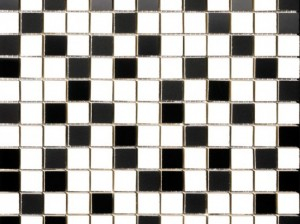
\includegraphics[height=8cm]{../../graphics/black_white_tile.jpg}
	\end{center}
\end{frame}

In presenting the first account, Aristotle asks us to imagine a visible compound composed of white and black parts, themselves too small to be visible. Since the compound is visible it must have some color. Since the white and black parts are too small to be visible, the color of the compound could not be either of these. So the compound must have some other kind of color. And it is the proportion of white and black components that determines the given chromatic hue. \change

\begin{frame}
	\begin{center}
		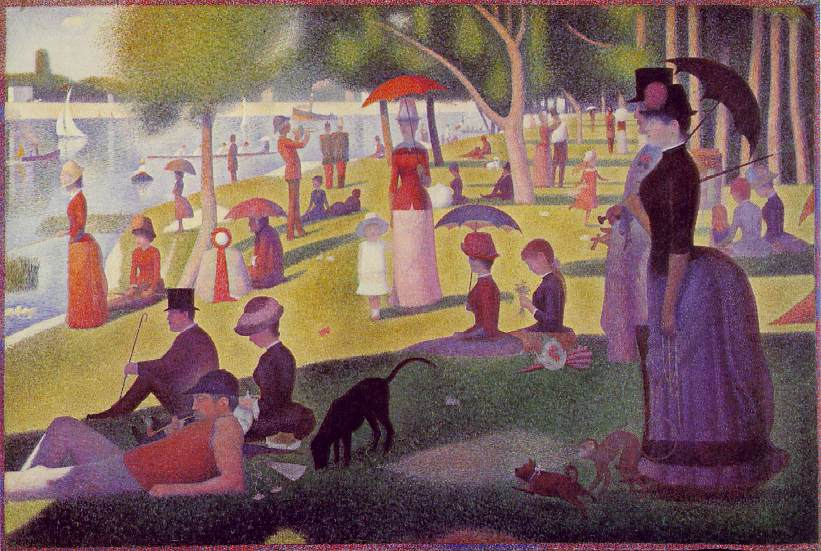
\includegraphics[height=7cm]{../../graphics/jatte.jpg}
	\end{center}
\end{frame}

Familiarity with pointillism and color halftone printing can obscure for us the real achievement in Aristotle's entertaining the possibility that the color of a compound can differ from the color of its parts. Pointillist paintings and color halftone prints have minute parts that differ in color from the painting or print as a whole at least when viewed from a suitable distance. Fascinated by the appearance of a color being influenced by adjacent colors, George-Pierre Seurat eventually paints the pointillist masterpiece, ``Un dimanche apr\`es-midi \`a l'\^Ile de la Grande Jatte'' over the course of two years beginning in 1884. Using only primary unblended pigments, including the newly available zinc yellow, these were distributed in small dots across the surface of the canvas giving rise to the appearance, at an appropriate distance, of a differently colored scene of Parisian suburbanites relaxing by the river Seine. The analogy is imperfect, however, in that the minute parts of the painting are merely too small to be seen from a suitable distance, where as the white and black parts of Aristotle's compound are too small to be seen at any distance.

A consequence of the juxtaposition model is that it is possible to see the color of a whole without seeing the distinct colors of its parts. That, however, is only intelligible set against a background conception of perception as providing a \emph{partial} perspective on the natural environment. Not only is perception partial in the sense that there are properties of an object not perceptually available (objects may have unobservable aspects), not only is perception partial in the sense that some sensible qualities of an object may be occluded from view (the backs of objects are colored as well), but perception is also partial in the sense there are sensible qualities of an object that are not determined by a given perception. If one can see the blue of a whole while failing to see that it is partly white and partly black, then one can see some if not all of an object's chromatic features. This is only possible if perception is partial in something like the sense described above. 

Aristotle rejects the juxtaposition model partly on the grounds that it posits colored objects too small to be seen (\emph{De Sensu} \textsc{iii} 440\( ^{a} \)21--25). Such parts would have magnitude and yet would be invisible. But, according to Aristotle, there are no invisible magnitudes. Every magnitude is visible from some distance. And while the color of some wholes dissolve upon closer inspection, such as Seurat's masterpiece, not all do. There are some surfaces that retain their color no matter how closely we look. So the juxtaposition model is implausibly revised to claim instead that the colors of compounds are determined by the juxtaposition of minute white and black parts that are normally not visible. It is open to ready empirical disconfirmation when we fail to discover these black and white parts despite our best efforts. \change

\begin{frame}[t]\frametitle{Overlap}
	\begin{center}
		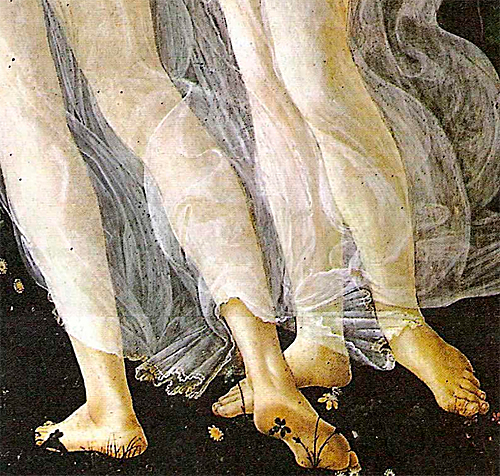
\includegraphics[height=8cm]{../../graphics/botticelli1.jpg}
	\end{center}
\end{frame}

The second model that Aristotle considers works not by means of juxtaposition, but by means of overlap (number 9 on your handout):
\begin{quote}
	Another theory is that they appear through one another, as sometimes painters produce them, when they lay a colour over another more vivid one, \emph{e.g.}, when they want to make a thing show through water or mist; just as the sun appears white when seen directly, but red when seen through fog or smoke. But on this view too the multiplicity of colours will be explained in the same way as before; for there will be some definite ratio between the superimposed colours and those below. (\emph{De Sensu} \textsc{iii} 440\( ^{a} \)7--15)
\end{quote}
Perhaps colors are not so much juxtaposed as they are overlapping. The overlapping colors, however, are perceptually penetrable at least to some degree---they appear through one another. Suppose one color overlays another color. If the overlaying color is perceptually impenetrable, if it determines a visual boundary through which nothing further could appear, the underlying color would be occluded, and this would not be a method of color combination. Moreover, it cannot be perfectly transparent. If the overlaying color were perfectly transparent, it would be wholly receptive of the underlying color, and, again, this would not be a method of color combination. For the overlap model to work, at least the overlaying color must be imperfectly transparent. The overlaying color's contribution to the resulting chromatic appearance consists, in part, in the visual resistance it offers. Moreover, the ratio of the overlapping colors that results in the novel color is partly determined by the degree of visual resistance offered by the overlaying color.

The painting analogy is arguably a deliberate echo of Empedocles (DK \textsc{b}23). As in the Emepedoclean fragment, the method of color combination deployed by the painters is overlaying colored washes---the method that Plutarch attributes to Apollodorus and is characteristic of Greek four-color painting more generally. Aristotle's choice of depicted content further emphasizes this: He draws our attention to how a painter might depict something appearing through water or mist by overlaying a wash of some appropriate color. Here perceptually penetrable washes of pigment are the means of representing something that is itself perceptually penetrable---the water or mist through which the object appears. He draws our attention to the imperfectly transparent subject matter as a way of emphasizing the imperfectly transparent means of representing that subject matter. \change

\begin{frame}
	\begin{center}
		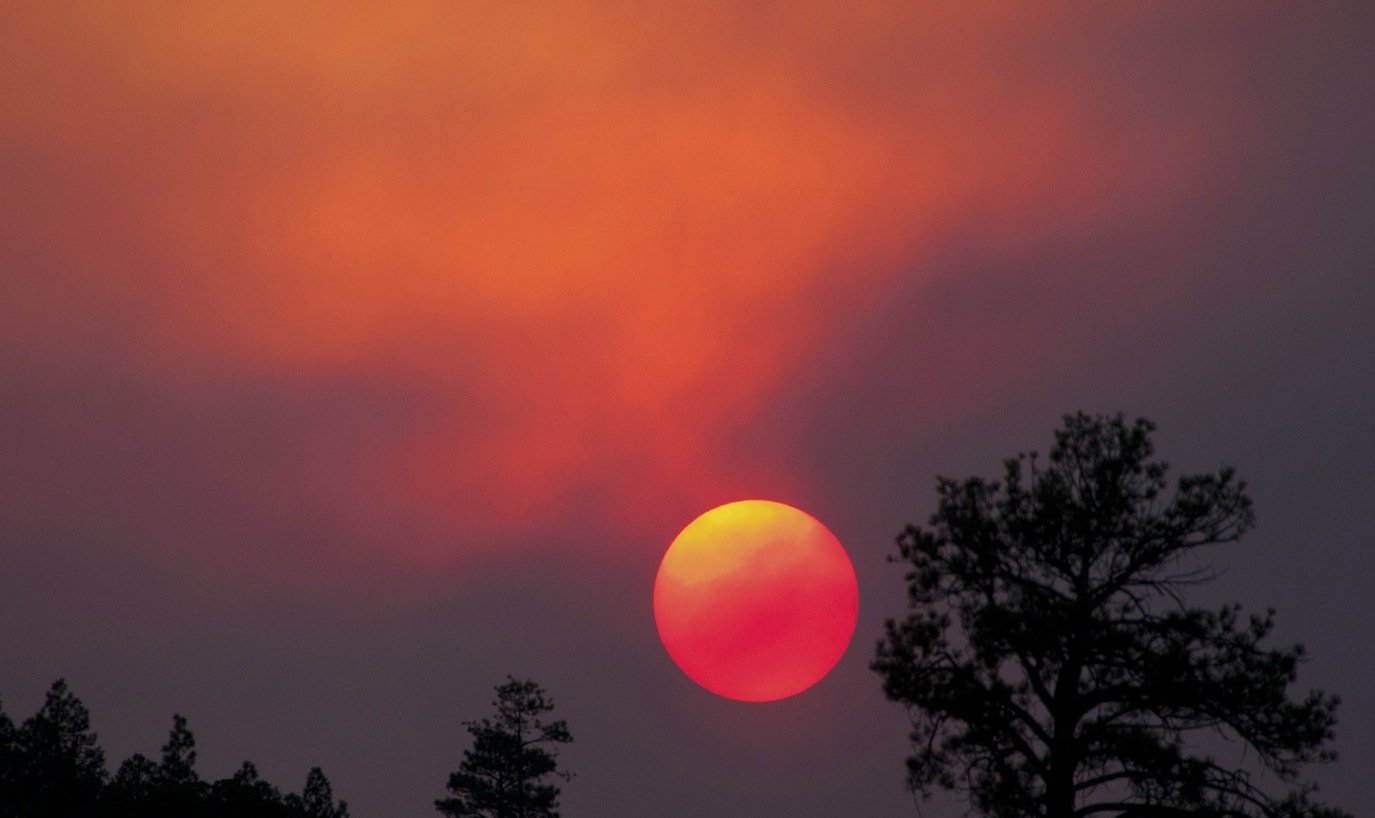
\includegraphics[height=6cm]{../../graphics/red_sun.jpg}
	\end{center}
\end{frame}

The sun seen through a fog or cloud of smoke is Aristotle's second analogy. The sun is white, and the smoke is black. And yet when the cloud of smoke is superimposed over the sun, it gives rise to a crimson appearance. If the black of the smoke were perceptually impenetrable, if it determined a visual boundary through which nothing further could appear, then the white of the sun would have been occluded. If on the other hand, the smoke were perfectly transparent, it would be wholly receptive to the white of the sun. For the analogy to work, the smoke must be imperfectly transparent. The blackness of the smoke contributes to the resulting chromatic appearance, in part, by the visual resistance it offers. Though it remains receptive of the white of the sun, otherwise it would be opaque, the darkness of the smoke resists perceptual penetration insofar as it can. The resulting proportion of light and dark presented to the organ of sight is determined in part by the degree of perceptual penetrability of the smoke. And it is the ratio of light and dark that determines the sun's crimson appearance.

The overlap model doesn't postulate invisible magnitudes, and so is not subject to the difficulty facing the juxtaposition model. Moreover, it retains what is by Aristotle's lights the salutary doctrine that chromatic hues are determined by a ratio of light and dark. However, Aristotle rejects the overlap model in favor of a model that works by mixture (number 10 on your handout):
\begin{quote}
	\ldots\ for it is not from afar only (but not from near at hand) that the color of mixed bodies seem uniform, but from all distances. (\emph{De Sensu} \textsc{iii} 440\( ^{b} \)16--18)
\end{quote}
This can initially strike one as an odd response. Indeed, the complaint seems best directed at an alternative to the juxtaposition model that does not posit invisible magnitudes, but rather magnitudes too small to be seen in normal circumstances. Think again of pointillist painting. The color of the painting only seems uniform at a suitable distance but dissolves into differently colored parts when near at hand. But not all visible particulars are like that. A laurel leaf will look green no matter how close you look at it and still count as looking. What is puzzling is how this objection could get a grip on the present model. How can the variability of color with distance arise by means of overlap?

Consider the sun seen through a cloud of smoke. Suppose the black particulate matter is uniformly distributed in the volume of the cloud. Then the degree to which the sun's brilliance is decreased will depend on the depth of the intervening volume. Holding fixed the density of the particulate matter, a greater volume of smoke will result in a greater reduction in the sun's brilliance than would result had the sun been seen through a smaller volume. A smaller volume of smoke, with the same density, while dark, would not be as dark as the greater volume. Indeed, seen through the smaller volume of smoke, the sun would not appear crimson, but orange, say. But this is just the variability of color with distance that Aristotle objects to.

Aristotle's complaint is that ``it is not from afar only \ldots\ that the color of mixed bodies seem uniform, but from all distances.'' There are two ways to understand this objection. On the first understanding, what's uniform is the color appearance presented by the particular when viewed from all distances from which its color can be seen. On the second understanding, what's uniform is the color the particular appears to have at all distances from which its color can be seen.

On the first understanding, the overlap model is at best an overgeneralization of a special case. The color appearance of at least some particulars are relatively uniform at any distance. The example of the laurel leaf looking green no matter how close you look at it may encourage this thought. It is true that proximity to the laurel leaf does not reveal it to be partly white and partly black. But that is not to say that the green of the leaf appears the same way at every distance from which it can be seen. Indeed, it is unobvious that there are any such particulars. The son of Diares looks like a white speck when seen from a distance in the way that he does not closer up. The problem with the present understanding is not just that it seems false, but that it can be seen to be false by reflecting on Aristotle's own examples. 

On the second understanding, what remains uniform is the perception of the particular's color despite that color's appearance varying with the distance from which it is viewed. On this understanding, that the color of a particular seems uniform at all distances just is seeing the constant color of the particular at any distance at which it is visible despite its appearance varying with the circumstances of perception. On this second understanding, then, the overlap model is inconsistent with an aspect of color constancy. On the overlap model, color varies with distance, but one can at least sometimes see a particular's unchanging color despite its color appearance changing in changing one's point of view.

The fundamental problem with the present account is that it too closely models color combination in terms of the appearance of a color through an imperfectly transparent medium with a given volume color. The surface color of a figure can be seen through water or mist, just as the radiant color of the sun can be seen through a cloud of smoke. In seeing a colored particular through a colored medium, the resulting chromatic appearance is partly due to the surface or radiant color of the particular and partly due to the volume color of the medium. But this is at best an account of how colors jointly combine to determine a chromatic appearance, and not an account of color combination. The way in which the overlap model runs afoul of color constancy is a symptom of this. That color appearances vary with distance was mistaken for the colors themselves varying with distance. Once the mistake is made, there is no color that persists as the object of visual awareness throughout the flux of sensory appearances that arises in changing one's point of view. \change

\begin{frame}[t]\frametitle{Mixture}
	\begin{center}
		
\includegraphics[height=8cm]{../../graphics/mixing.jpg}
	\end{center}
\end{frame}

Larger philosophical concerns are at work in Aristotle's claim that it is the ratio of light and dark in a \emph{mixture} that determines chromatic hues. % 

According to Empedocles, the combination of the ``roots'' or elements operates on the model of juxtaposition. The divine glues of harmony bind the elements not by mixture, but as small pieces standing next to each other touching (DK \textsc{b}96). It is in these terms that Empedocles sought to explain the growth and decay of compound bodies. What mortals describe as ``growth'' and ``decay'' are really the result of the combination and separation of unalterable, ungenerated, and imperishable elements (DK \textsc{b}8). While Empedocles resisted in this way the full thrust of Parminedean skepticism about generation and corruption, the concessions he makes to Parmenides distinguishes his view from sixth century \textsc{bc} thinkers as yet untouched by Parmenidean doubts. Thus Kahn remarks that ``The fundamental difference between the sixth and fifth centuries lies not in the abandonment of monism for plurality, but in the passage from a world of birth and death to one of mixture and separation.'' 

On Aristotle's view, the Emepdoclean tetrad---water, earth, air, and fire---are only elements so-called. Strictly speaking, elements are the simple primary ingredients of a compound (\emph{Metaphysics} \( \Delta \) 1014\( ^{a} \)26ff). So understood the real elements are the primary opposites: Hot, Cold, Dry, and Wet. The so-called elements, water, earth, air, and fire, are the result of the combination of these opposing principles. Thus water is Cold and Wet, earth is Cold and Dry, air is Hot and Wet, and fire is Hot and Dry. Since the Empedoclean tetrad are only elements so-called, they are subject to a cycle of transformation familiar from ancient times. In a passage self-consciously recounting the older view, Plato describes  (in number 11 on your handout) the cycle of elemental transformation. Aristotle regards the continuous transformation of the Empedoclean tetrad into one another as an established fact of observation. So conceived, they could not be the Parmenidean beings that Empedocles understands them to be. The combination of the so-called elements, is no longer understood in terms of the juxtaposition of unaltering, ungenerated, and imperishable beings. Water, earth, air, and fire transform into one another and in so doing interfuse. And it is complete interfusion that is mixture properly so-called. In a compound body composed of different items from the Empedoclean tetrad, the so-called elements combine by interfusing, at least to some degree, that is, by mixture. With respect to elemental composition, Aristotle's doctrine thus represents a return to the sixth century \textsc{bc} view.

Aristotle's preferred model of the generation of the hues should be understood set against this larger reaction to Parmendiean skepticism about growth and decay. It is because he regards combination and separation as an imperfect surrogate for growth and decay (\emph{On Generation and Corruption} \textsc{i} 10), that he understands elemental composition instead in terms of mixture. And it is natural, if not inexorable, that he should have a parallel understanding of chromatic composition. That light and dark are the primary colors is an ancient doctrine, of Homeric roots, that Parmenides and Empedocles share. Aristotle follows them in this. Moreover, Aristotle takes over from Parmenides and Empedocles the idea that light and dark are contraries that constitute the extreme ends of an ordered range of sensible qualities. Moreover, he emphasizes Empedocles' contribution to this tradition in claiming that it is the ratio of light and dark when combined that determines an intermediary color. Aristotle, however, departs from Empedoclean doctrine precisely in the method of combination. Aristotle understands the combination of light and dark in terms of a conception of mixture at home in pre-Parmenidean natural philosophy, in the sixth century \textsc{bc} world of birth and death. 

Any assessment does well to distinguish separable strands in this ancient tradition. I suspect that skepticism about it is due in large part to an intuitive recognition of its inadequacy as an account of color similarity. Fortunately, the ancient tradition does not consist entirely of claims about color similarity; at the heart of the ancient view is a claim about the explanatory priority of cosmic Fire. That a proportion of light and dark determined by the presence and activity of fire explains a particular's color is echoed by modern reflectance theories that maintain that it is the amount of light reflected at each of the wavelengths of the visible spectrum that determines a particular's color. The more general idea, free from the anachronistic intrusion of the Newtonian spectrum, is that color is way of affecting light. (In the traditional post-Lockean vocabulary, color is not so much a secondary quality as it is a tertiary quality.) This idea is enshrined in Aristotle's definition of color as the power to move what is actually transparent, that is, what is illuminated by the presence and activity of the fiery substance.

\end{document}